\section{CR Alternativi: CTFBox}\label{cr-alternativi-ctfbox}

CTFBox è un Cyber Range perfetto per organizzare CTF di tipo
Attack/Defense, dove ogni team ha una macchina con uno o più servizi
vulnerabili da difendere, mentre si attaccano i servizi esposti sulle
macchine avversarie per recuperare le flag. Durante il gioco, ogni team
deve fare attenzione a non rompere i propri servizi, mantenendo un'alta
percentuale di SLA. Una SLA bassa comporta una penalità in termini di
punteggio. \footnote{\label{fn:ref_7}https://ctfbox.domy.sh/}

Fa uso di \textbf{Docker} per gestire i servizi essenziali del gioco (e
che costituiscono quindi CTFBox), mentre \textbf{Incus} viene utilizzato
per gestire l'esecuzione delle macchine virtuali o dei container dei
team (Figura \ref{fig:ctfbox-architecture}).


\begin{figure}[!htbp]
  \centering
  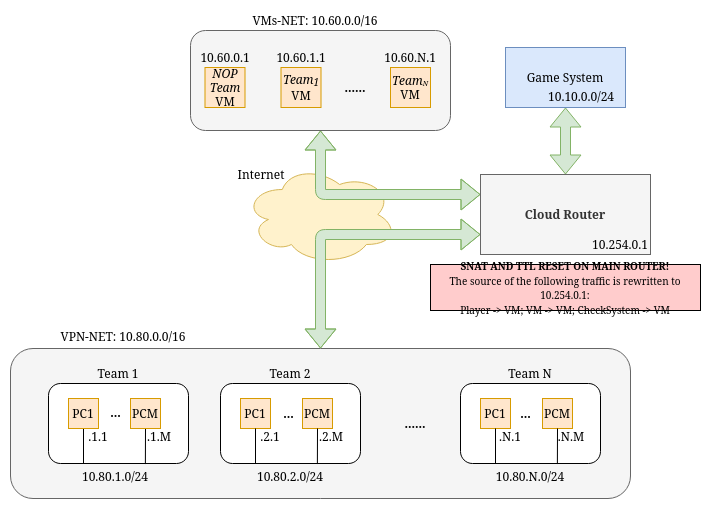
\includegraphics[width=0.68\linewidth,height=0.30\textheight,keepaspectratio]{src/images/ctfbox-architecture.png}
  \caption[Architettura di CTFBox]{Architettura modulare di CTFBox}
  \label{fig:ctfbox-architecture}
\end{figure}


\textbf{Router}: è un container Docker, che gestisce le configurazioni
della rete WireGuard, permettendo ai giocatori di connettersi alla rete
di gioco. Controlla le regole di routing sulla rete, e governa la
transizione della rete tra 3 stati diversi:

\begin{itemize}
\tightlist
\item
  \passthrough{\lstinline!freeze!}: in questo stato, nessuno può
  accedere alle macchine vulnerabili
\item
  \passthrough{\lstinline!lock!}: in questo stato, ogni team può
  accedere solo alla propria macchina vulnerabile.
\item
  \passthrough{\lstinline!unlock!}: in questo stato, la rete è
  completamente aperta, i team possono attaccare le macchine avversarie.
\end{itemize}

\textbf{Game System}: è un container Docker, che agisce da cervello
centrale per la gestione del gioco.

\begin{itemize}
\tightlist
\item
  Gestisce lo stato della rete (freeze/lock/unlock), comunicando i
  cambiamenti al router.
\item
  Mantiene il database delle flag, e calcola i punteggi per ogni team.
\item
  Coordina i Checkers, ossia i worker che interrogano i servizi dei team
  ad ogni tick.
\end{itemize}

In CTFBox, ad ogni tick (ossia ogni round di gioco), le flag vengono
rigenerate su ogni macchina, per ogni servizio vulnerabile, e registrate
nel database. L'obiettivo di un team in una competizione Attack/Defense
strutturata in questo modo è di attaccare più volte lo stesso servizio
sulle macchine avversarie, per recuperare quante più flag possibili,
finché le difese avversarie non bloccano gli attacchi.

\textbf{Checkers}, ad ogni tick (o round) fanno due cose:

\begin{enumerate}
\def\labelenumi{\arabic{enumi}.}
\tightlist
\item
  Interrogano tutti i servizi vulnerabili attivi, e determinano la
  percentuale di SLA per ogni team.
\item
  Installano le nuove flag sui servizi vulnerabili.
\end{enumerate}

Ogni membro del team, ha la sua configurazione \textbf{WireGuard} per
connettersi alla propria macchina e per raggiungere le macchine
avversarie. Ad ogni giocatore che si connette viene assegnato un
indirizzo nella sottorete \passthrough{\lstinline!10.80.team\_id.0/24!}
mentre le macchine dei team si trovano nella sottorete
\passthrough{\lstinline!10.60.0.0/16!}.

Dunque CTFBox si rivela essere un ottimo sistema per gestire
competizioni Attack/Defense e per regolare l'accesso alle macchine, ma
la sua architettura non si applica in contesti in cui vorremmo solo
assegnare ad ogni team un insieme di macchine vulnerabili il cui stato
verrà poi verificato da un oracolo.

Sia CTFBox che BlueAgent usano WireGuard ed Incus per gestire le
connessioni dei partecipanti e le macchine dei vari team.

Tuttavia CTFBox gestisce intere macchine virtuali mentre BlueAgent per
design gestisce di default solo container di sistema.

Di seguito sono riassunte le principali differenze tra CTFBox e
BlueAgent:

\begin{longtable}[]{@{}
  >{\raggedright\arraybackslash}p{(\linewidth - 4\tabcolsep) * \real{0.3333}}
  >{\raggedright\arraybackslash}p{(\linewidth - 4\tabcolsep) * \real{0.3333}}
  >{\raggedright\arraybackslash}p{(\linewidth - 4\tabcolsep) * \real{0.3333}}@{}}
\toprule\noalign{}
\begin{minipage}[b]{\linewidth}\raggedright
Caratteristica
\end{minipage} & \begin{minipage}[b]{\linewidth}\raggedright
CTFBox
\end{minipage} & \begin{minipage}[b]{\linewidth}\raggedright
BlueAgent
\end{minipage} \\
\midrule\noalign{}
\endhead
\bottomrule\noalign{}
\endlastfoot
\textbf{Modello di Gioco} & Attack \& Defense competitivo tra team &
Defensive / Blue Teaming \& Patching \\
\textbf{Virtualizzazione} & Macchine Virtuali / Container eterogenei &
Container di sistema dedicati (Incus) \\
\textbf{Topologia di Rete} & Subnet condivisa aperta
(\passthrough{\lstinline!10.60.0.0/16!}) & LAN virtuale dedicata e
isolata per team \\
\textbf{Meccanismo di Verifica} & Polling periodico su rete di gioco
(Checkers a tick) & Esecuzione su clone CoW ZFS in rete OVN isolata \\
\textbf{Invisibilità della Verifica} & Assente (il traffico dei checker
viaggia su rete condivisa) & Totale (l'oracolo esegue in una rete SDN
separata) \\
\textbf{Calcolo del Punteggio} & SLA di uptime dei servizi e flag rubate
& Rilascio della flag a seguito di patch corretta \\
\end{longtable}
